
\section{Flavor}\label{sec:flavor}

\renewcommand{\kapitelautor}{Autor: Philip Jankovic}

\subsection{Definition Falvor}\label{subsec:wichtigkeit-des-flavours}
%TODO BILDER
%
Mit Flavor, im Bezug auf Kartenspiele, ist gemeint, welche Geschichten und Hintergründe hinter den einzelnen Karten stecken.
Es verknüpft die Optik, den Namen und die Funktion mit der Idee bzw dem Konzept der Karte.
Flavor gibt jeder Karte etwas Eigenes, was sie von anderen unterscheidet.

"Flavor is the Soul of the game"\zit{soulOfTheGame}


Flavor kann auf verschiedene Arten auftreten. Flavor kann in Karten und generell in Spielkonzepten/Regeln existieren.
Es verknüpft die Karten, das Setting, die Story und die Spielregeln. Grob kann ein Kartenspiel in Funktion und Flavor aufgeteilt werden.
Beide existieren zusammen und keines ist wichtiger als das andere.
Unter Funktion wird verstanden, wie das Spiel gespielt wird, was Regeln und Mechaniken einschließt.\zit{flavorAndFunction}


\subsection{Flavor durch Spielmechaniken und Spielmechaniken durch Flavor}\zit{subsec:flavour-durch-mechaniken}

Flavor und Funktion, zusammen also Spielmechaniken, sind das Erste, über das nachgedacht werden sollte wenn man ein Kartenspiel designed.
Flavor in den Spielregeln erlaubt Spielern, bereits vorhandenes Wissen im Spiel anzuwenden und das Spiel dadurch besser zu verstehen. \zit{flavorAndFunction}


In \FF ist das Spielfeld der Revolver. Vielen Spielern ist bereits bewusst, dass Bullets in einen
Revolver geladen werden. Da alle Karten Bullets sind, kann sich der Spieler denken, das die Karten in den Revolver geladen werden. Die Mechanik des Ladens
der Karten in das runde Spielfeld greift in den Flavor, der besagt, dass diese Karten Bullets sind und das runde Spielfeld
ein Revolver ist. Wären die Karten keine Bullets, sondern zum Beispiel Kreaturen und der Revolver kein runder Kreis,
der rotieren kann, wäre \FF nicht \FF, sondern ein anderes Spiel mit dementsprechend anderem Setting, kein Wild-West
Spiel und würde dementsprechend mit einem anderen Flavor verbunden sein.


Die Trommelrotation und das Abschießen von Bullets macht nur Sinn, da das Spielfeld ein Revolver ist.
Dass die Karten Bullets sind, macht nur Sinn, weil das Setting im Wilden Westen spielt und das Spielfeld ein Revolver ist.
Dass das Spielfeld ein Revolver ist, macht nur Sinn, da er nach rechts rotiert und die vorderste Karte rausschießt wenn er abgefeuert wird.
Ohne den Flavor sind die Spielregeln von \FF unnachvollziehbar und können ohne das andere nicht exestieren.


Anders gesagt, gibt der Flavor einem Kartenspiel, welches eigentlich nur ein abstraktes Konzept aus Nummern und Regeln ist,
an welche sich Menschen halten, damit ein Spiel zustande kommt, einen Grund für die Funktionalitäten und damit eine \quoted{Seele}.


Auch in \quoted{Magic the Gathering}, \quoted{Inscription} oder \quoted{Balatro} ist dieses Konzept sichtbar.

In \quoted{Magic the Gathering}
ist das Spielkonzept breit und umfangreich.
Das Setting ist nicht so streng definiert wie in \FF, was mehr verschiedene Spielmechaniken und Karten ermöglicht.
Dafür fühlt sich das Spiel manchmal nicht mehr an wie \quoted{Magic the Gathering},
was bei \FF durch die strikte Einhaltung der Mechaniken und der Karten, also Bullets und dem Revolver, nicht passieren kann.\zit{magicarena}


Der Flavor von \FF ist stark und das durchziehende Konzept der Bullets so konstant, dass das Spiel und seine Regeln immer
wiederzuerkennen sind. Ähnlich ist es bei \quoted{Balatro}, einem pokerinspirierten Rogue-lite Deckbuilding Spiel.
So wie die sammelbaren Karten in \FF Bullets sind, sammelt der Spieler in \quoted{Balatro} verschiedene Joker Karten.
Obwohl \quoted{Balatro} erst veröffentlicht wurde, als die erste Release-Version von \FF die Entwicklung bereits abgeschlossen hatte,
ist das Konzept von den verschiedenen und komischen Jokern von \quoted{Balatro} sehr ähnlich zu den verschiedenen und
komischen Bullets von \FF. \zit{balatro}


\quoted{Inscription} wiederum verfügt über weniger konstantes Kartendesign, auch wenn jede Karte ein anderes Tier darstellt,
legt dafür aber Wichtigkeit auf das Setting und die Stimmung, die das Spiel vermittelt. Durch Opfern von Karten können stärkere Karten
gespielt werden, was gut zu dem Horrorsetting passt. Auch Lebenspunkte werden abgerechnet durch herausgerissene Zähne und Augen.\zit{inscryption}


All diese Beispiele zeigen, wie Spiele aus demselben oder sehr ähnlichen Genre sich durch ihr Setting, Flavor und Spielmechaniken unterscheiden.


\begin{figure}[H]
    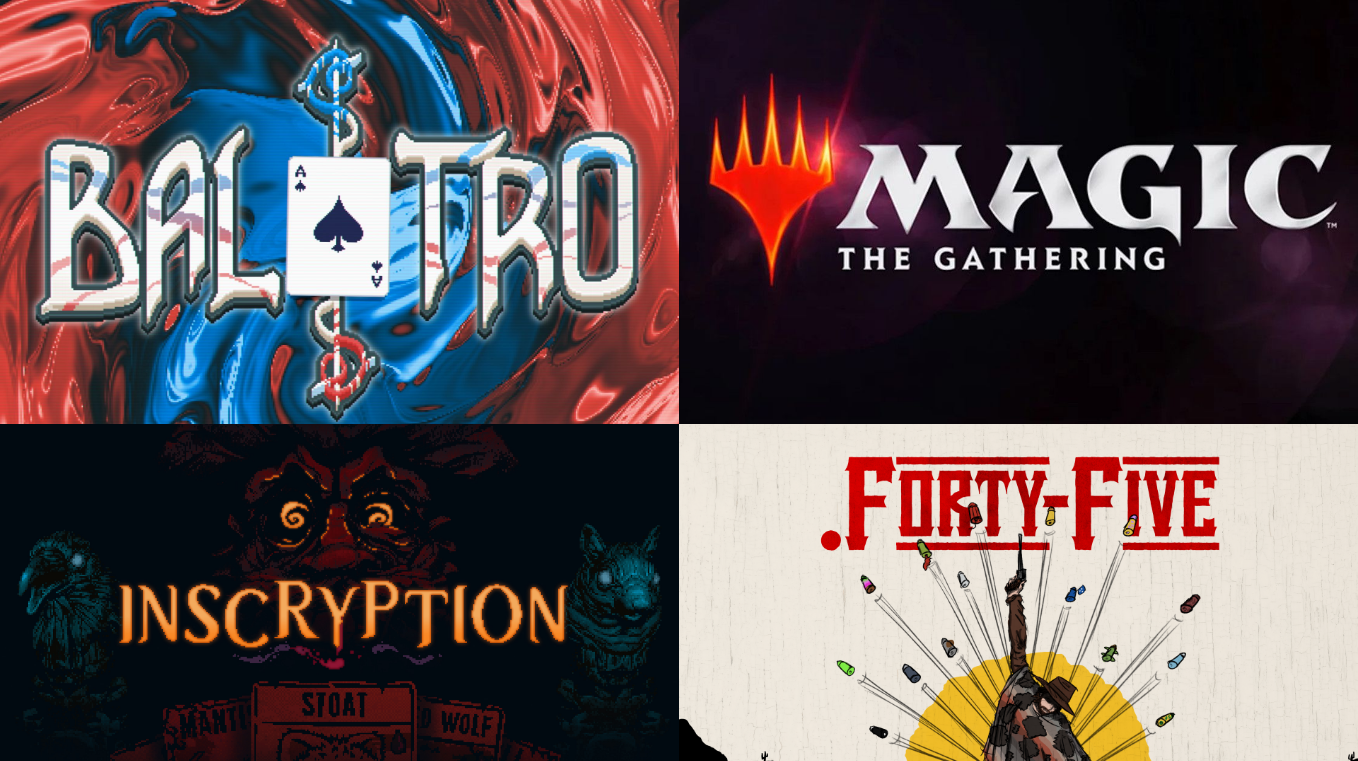
\includegraphics[width=\textwidth]{4games.png}
    \caption{Beispiel: vier verschiedene Deckbuilding Spiele}
\end{figure}


Die Erschaffung der Spielregeln und damit auch des Flavors von \FF gingen Hand in Hand miteinander.
Zuerst kam die Idee des Settings des Wilden Westens, dann das Spielkonzept. Mehr zu Methoden kann in \ref{methoden}
nachgelesen werden. Wichtig für dieses Kapitel ist, dass selbst nach zwei Jahren Arbeit und vielen Änderungen an Spielregeln,
das Grundkonzept noch immer das gleiche ist. Viele Karten, die zu Beginn der Entwicklung in Notizbüchern aufgezeichnet wurden, befinden sich
fast identisch noch immer im Spiel.



Spielmechaniken sind jedoch nicht das Einzige, in dem Flavor eine wichtige Rolle spielt.

\subsection{Cardflavor}\label{subsec:cardflavor}

Cardflavor ist der Flavor einzelner Karten.
Dazu gehört ihr Name, ihre Optik, ihr Effekt, wie der Effekt mit dem Namen der Karte zusammenhängt,
ihr Platz in der Welt und ihre Hintergrundgeschichte. Je nach Karte sind mehr oder weniger der genannten
Merkmale vertreten.


Zusätzlich zu dem Effekt der Karte, der sichtbar wird, wenn der Spieler über die Karte hovert, haben einige Karten zusätzlich einen sogenannten Flavortext.
Flavortexte sind zum Beispiel auch in \quoted{Magic the Gathering} vertreten und beschreiben die Welt der Spieles oder geben
Zitate von verschiedenen Charakteren in der Magic-Welt wieder.\zit{magicarena,soulOfTheGame}


Auf den Bullets von \FF kann ein Flavortext entweder Worldbuilding, ein Spruch, ein Witz oder eine Anspielung sein, die zur Karte passt.

%TODO bilder mit beispielen

\begin{figure}[H]
    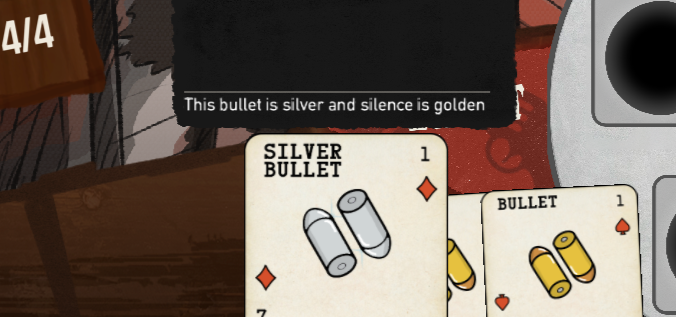
\includegraphics[width=50\%]{flavorscreen.png}
    \caption{Beispiel: Flavortext von "Silver Bullet"}
\end{figure}


Die zweite Art, einer Karte Flavor zu verleihen, ist es, den Karteneffekt an den Namen der Karte anzupassen.


In den meisten Kartenspielen ist das Ziehen von Karten ein großer Vorteil für einen Spieler, da eine größere Kartenauswahl
auch mehr Kontrolle bedeutet. Dies wird in den Communities umgangssprachlich als "Value" bezeichnet. \zit{whatsvalue}
Auch in \FF spielt Value eine große Rolle.
Da Value wertvoll für den Spieler ist, werden alle Bullets, welche Value durch das Zeihen von Karten erzeugen, einem
wertvollen Material zugeordnet, \zB "Gold Bullet" oder "Silver Bullet"

\begin{figure}[H]
    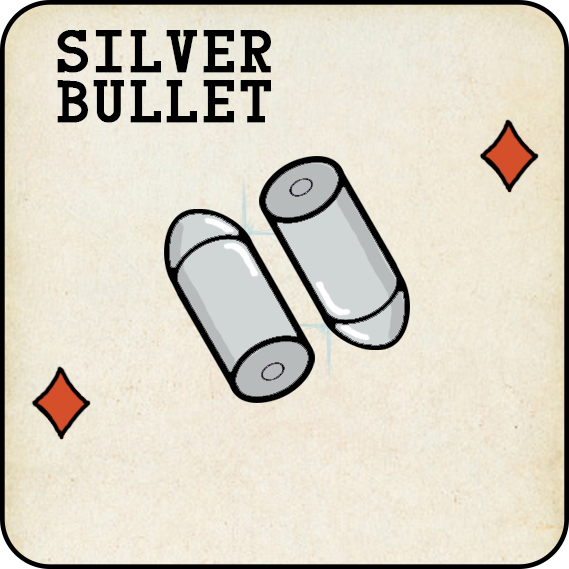
\includegraphics[width=50\%]{silverB.png}
    \caption{Beispiel: "Silver Bullet"}
\end{figure}

    \begin{figure}[H]
    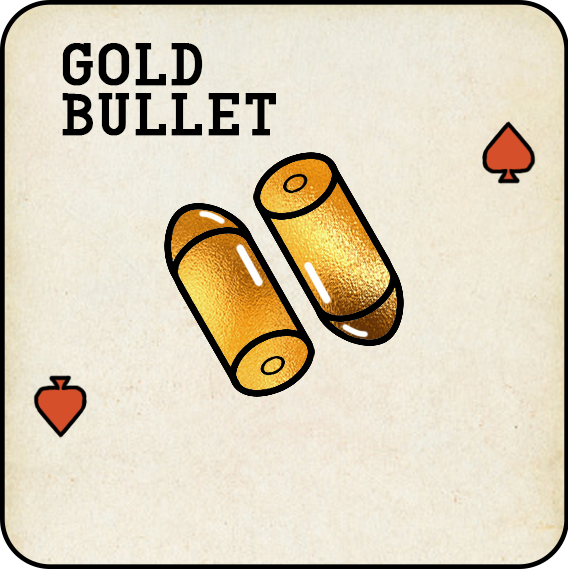
\includegraphics[width=50\%]{goldB.png}
    \caption{Beispiel: "Gold Bullet"}
\end{figure}



"Golddiggers Bullet" wiederum profitiert von der von den "wertvollen" Bullets erzeugten Value, da man durch "Golddiggers Bullet" Reserves bekommt,
wenn eine Karte gezogen wird. Sie wandelt also die Value erzeugt durch die wertvollen Bullets in Reserves um.
Ähnlich wie ein Goldgräber, der Gold findet und es anschließend gut verkauft.

\begin{figure}[H]
    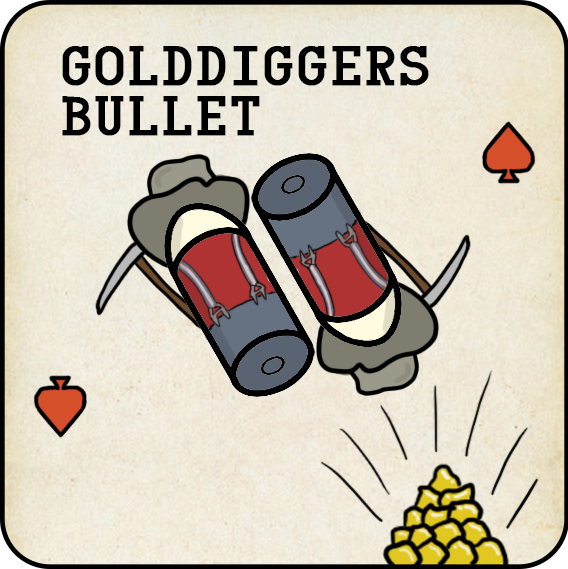
\includegraphics[width=50\%]{golddiggersB.png}
    \caption{Beispiel: "Golddiggers Bullet"}
\end{figure}

Auf einem ähnlichen Konzept basiert "Gravediggers Bullet", die davon profitiert, wenn Karten "sterben", also zerstört werden.


\begin{figure}[H]
    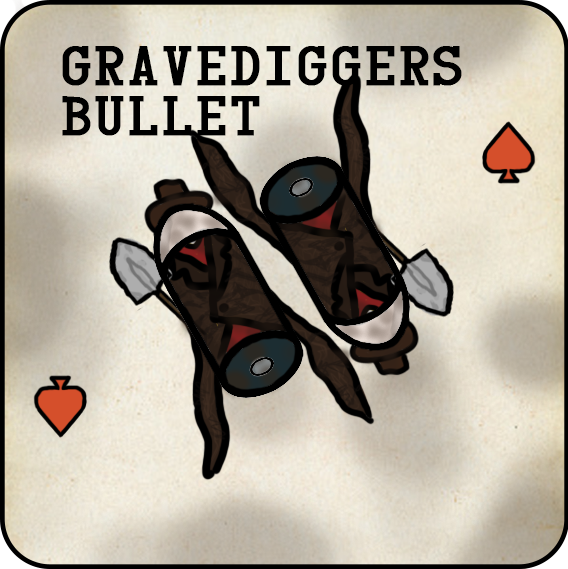
\includegraphics[width=50\%]{graveB.png}
    \caption{Beispiel: "Gravediggers Bullet"}
\end{figure}


Diese Flavor Effekte der Karten ziehen sich durch das ganze Spiel und nutzen die Spielmechaniken um die Konzepte der Bullets umzusetzen.
"Rotten Bullet" \zB verliert mit jedem Mal, die sie im Revolver rotiert, einen Dmg ihrer Dmg-Value, da sie langsam "verrottet".


"Gold Bullet" wird mit der Zeit immer mehr wert, da sie, wenn sie abgeschossen wird, also "verkauft" wird, x Karten zieht,
wobei x die Nummer der durchlaufenen Revolverrotationen von "Gold Bullet" ist. Es werden also Eigenschaften von Gold,
nämlich dass es immer mehr wert wird, je länger es in Besitz ist, in die Spielmechaniken von \FF integriert.


Cardflavor ist unter anderem wichtig für das Kartenspiel, da damit Unglaubwürdigkeiten aus dem Weg geräumt werden.
Cardflavor ist nicht bei allen Bullets gleich stark ausgeprägt. Dennoch muss ein gewisser Grundzusammenhang zwischen dem
Kartennamen und dem Effekt existieren. Ein Beispiel dafür wäre, dass eine Feuer Bullet irgendwas mit Feuer zu tun hat und
nicht den Himmel Frösche regnen lässt, übertrieben ausgedrückt.


Jeder Teil des Spiels sollte im besten Fall vor lauter Flavor strotzen, nicht nur die einzelnen Karten oder Spielmechaniken.



\subsection{Flavor everywhere}\label{subsec:keinTeildesSpielesOhneFlavor}

Wie in fast allen Bereichen des menschlichen Lebens heutzutage gewinnen KI-Modelle immer mehr Raum. Bei der Entwicklung von \FF war es dem Team wichtig,
dass sich das Spiel auch tatsächlich so anfühlt, als wäre es von Menschen für Menschen entwickelt worden.
Der Flavor und die kleinen Eigenheiten von \FF sollen dazu beitragen.
Das ganze Spiel ist voll mit Anspielungen, Inspirationen von anderen Medien und kleinen Sprüchen oder Witzen.
Das unterstreicht, wie wichtig es ist, dass der beschriebene Flavor konstant im ganzen Spiel zu finden ist.
Beispiele dafür sind die Encounter Modifier, welche auf die Spielmechaniken
angepasst wurden oder die eigens für das Spiel erstellte Schrift, die immer wieder im Spiel zu finden ist. Auch Ortsnamen
haben oft ein Wortspiel mit "Bullet" wie zum Beispiel "Tabu Letter Outpost" oder "Aqua Balle".


\subsection{Storytelling und Worldbuilding}\label{subsec:storytellingUndWorldbuilding}

\FF spielt in einer fiktionalen Version der USA, in der sogenannten Frontier. Gut 40 Jahre vor den Ereignissen von \FF
entdeckte ein Reisender die Frontier, die von dem einheimischen Stamm der Onathahans bewohnt wurde. Heutzutage ist die Frontier
eine scheinbar gesetzlose Zone, voll mit Outlaws und Individuen, die ihr Glück in der Frontier finden wollen.
Aus unbekannten Gründen sind verhexte Bullets in der Frontier verteilt. Ziel der Outlaws ist es, diese Bullets zu Geld
zu machen oder zum eigenen Vorteil zu nützen.


Was genau vor 40 Jahren vorgefallen ist und was mit den Onathahans
passiert ist, wird im Laufe des Spiels durch Flavortexte und Dialoge erklärt. Wenn der Spieler die Texte liest,
was ihm jedoch freigestellt ist, kann er die einzelnen Puzzlestücke zusammensetzen und damit die Welt von \FF kennenlernen.
Die Flavortexte auf den Karten können aufgrund der zufälligen Reihenfolge, in der der Spieler sie zu Gesicht bekommt, in beliebiger Reihenfolge gelesen werden.


Der Ansatz nennt sich "nicht lineares Storytelling" und ist zum Beispiel auch in \quoted{Magic the Gathering} zu finden.\zit{nonlinearstorytelling, magicarena}


Die Flavortexte der Bullet bieten dem Spieler Informationen über die Ereignisse der Vergangenheit und die Mysterien,
die die Frontier und die Bullets umgeben. Dialoge mit Charakteren liefern jedoch Informationen über den Handlungsstrang,
der sich in der Gegenwart abspielt. Dazu gehört auch \zB der Governor, der großes Interesse am Sammeln der verhexten Bullets hat.


Jede Story-Interaktion in \FF ist freiwillig und kann daher ignoriert werden, falls der Spieler kein Interesse an der Story hat.


Das Worldbuilding ist jedoch über das ganze Spiel verteilt. Bullets, welche den Revolver nach links, statt nach rechts drehen,
werden mit den Onathahans in Verbindung gebracht, welche von Außenstehenden einfach nur Hexen genannt werden.
Auch Orte und Biome werden von der Story beeinflusst, wie zum Beispiel Salem, die damalige Heimat der Onathahans, oder Aqua Balle,
der Eingang zur Frontier.


Die bereits erwähnte Schrift stellt die Schrift der Onathahans dar, um dem Worldbuilding mehr Glaubwürdigkeit zu geben,
ähnlich wie J.R.R. Tolkien eine eigene Sprache für Elben in seinem Meisterwerk "Herr der Ringe" entwickelte. \zit{elbenSprache}

% resets author
\renewcommand{\kapitelautor}{}
